\documentclass[]{article}
\usepackage{siunitx}
\usepackage{hyperref}
\usepackage{float}
\usepackage{graphicx}
\usepackage{dcolumn}
\usepackage{subcaption}
\usepackage[english]{babel}
\usepackage[backend=biber,style=numeric]{biblatex}
\usepackage[utf8]{inputenc}

\DeclareSIUnit\day{d}

\addbibresource{proposal.bib}

%opening
\title{Analyzing the Light Curve of DQ Cephei}
\author{Miles Lucas and John Brandon}
\date{\today}
\begin{document}

\maketitle

%______________________________________________________________________________

\begin{abstract}
	We seek to characterize the light curve of the $\delta$-scuti type variable star DQ Cephei. In order to do this we want to take four hours worth of exposures to capture two full periods of data. We want to use differential photometry using two reference stars for every image. We will use either a classic or a Lomb-Scargle periodogram to determine the period of variation.
\end{abstract}

%______________________________________________________________________________
\section{Equipment and Observations}
	We request use of the 8-inch Meade reflector telescope along with a 2x focal length extender for use with the CCD to increase its field of view. Our estimated period is around \SI{2}{\hour} and we want to capture as much data as possible. We want at least 4 hours of data and we think the best course of action would be to take exposures in 4 hour sessions over the course of two or three sessions. 
	
	\autoref{fig:staralt} shows that we will be able to see the star and have a reasonable airmass over this time period. Mid October shows promise for observations. Our most preferred date is \date{18 October 2017} due to the new moon. Our star is fairly distant from the moon, thankfully, so we do not have issues even if the moon is up, so other weeks work well, too. \autoref{tab:info} contains info about the star of interest and the reference stars for the differential photometry.
	\begin{table}[]
		\centering
		\caption{Information about target and reference stars}
		\begin{tabular}{rrrrrr}
			\hline
			Object & Type &            RA &                DEC &                      V &                        Ref \\ \hline\hline
			DQ Cep &  *dS & 20 57 48.6082 & \ang{55;29;15.602} & \SIrange{7.40}{7.48}{} & \autocite{1971GCVS3.C......0K} \\
			HD 235411 &    * & 20 57 31.1094 & \ang{55;31;38.697} &     \SI{9.76\pm0.03}{} &  \autocite{2000AA...355L..27H} \\
			HD 200017 &    * & 20 58 27.2026 & \ang{55;39;00.459} &     \SI{8.20\pm0.01}{} &  \autocite{2000AA...355L..27H} \\ \hline
		\end{tabular}
		\label{tab:info}
	\end{table}

%______________________________________________________________________________
\section{Scientific Justification}
	The goals of this project are to find the variation period of DQ Cep. We plan to do this by taking many images of the source with two reference objects (\autoref{fig:map}, \autoref{tab:info}). Each image will have an exposure that appropriately captures the dynamic range of the star, seeking about \num{40000} pixel count max for each image\footnote{Our SBIG CCD camera has a maximum value of around \num{65000} pixel counts}.

	In between each exposure, we should have a small break (\SI{10}{\second}) in order to realign the image if the objects start to drift out of frame. Through taking practice images and discussion we have concluded on using CCDops5's autograb script to take \SI{15}{\second} exposures with the \SI{10}{\second} break is most efficient. Autograb takes number of images as a parameter so we can take our total observation time and divide it by the time per image (\SI{25}{\second}) to determine that parameter. Because we want to use autograb, we are limited to taking images in only one photometric filter, which is fine. Lastly, we will have to take at least five dark frame images at our chosen exposure time for subtraction later on.


%______________________________________________________________________________
\section{Technical Justification}

	Previous experiments done using the same telescope and SBIG CCD have shown that differential photometry can be accurate to around \SI{0.01}{mag}. Because our expected magnitude range is \SI{0.08}{mag} we wanted to be sure a difference could be seen. Another important factor is having reliable reference stars in the same frame as the target star to enable differential photometry. To accomplish this, we need to use a focal length extender which effectively doubles our field of view (halves our magnification). We can then capture two reference stars, HD 235411 and HD 200017 in each frame, shown in \autoref{fig:map}.
	
	To showcase the precision we have already taken a preliminary dataset that shows a difference in the magnitudes. Each of the images was taken with a \SI{15}{\second} exposure and a \SI{10}{\second} break to allow manual repositioning if needed. This proved to be an effective method because over 90\% of our practice images turned out sharp of the 100 we took.
	
	With theses images, we were able to see a clear difference over time for our variable star. \autoref{fig:mags} shows an upward trend. We tried fitting a one term Fourier model (a simple sine wave) but it is very hard to get the frequency without having at least two relative extrema.
	
%______________________________________________________________________________
\section{Analysis Plan}

	The analysis pipeline will require processing approximately 600 images. This will require efficient programs, like AstroImageJ, which allow calculations on large image sequences. Using AstroImageJ we can dark subtract every image and perform differential photometry. 
	
	This photometry data will then be used to fit our variable model. Right now, we are leaning toward the use of a Lomb-Scargle periodogram, although a classical periodgram may work fine as well due to constant acquisition rate. \textcite{2017arXiv170309824V} gives an in-depth analysis of different variability modeling methods that will help us choose our final method for period-finding. Once we have established a good period for us to work with, we will fold the data into a period light curve.
	

%______________________________________________________________________________


\printbibliography

%______________________________________________________________________________
\newpage
\appendix
\section{Figures}
\begin{figure}[H]
	\centering
	\begin{subfigure}[]{.45\textwidth}
		\centering
		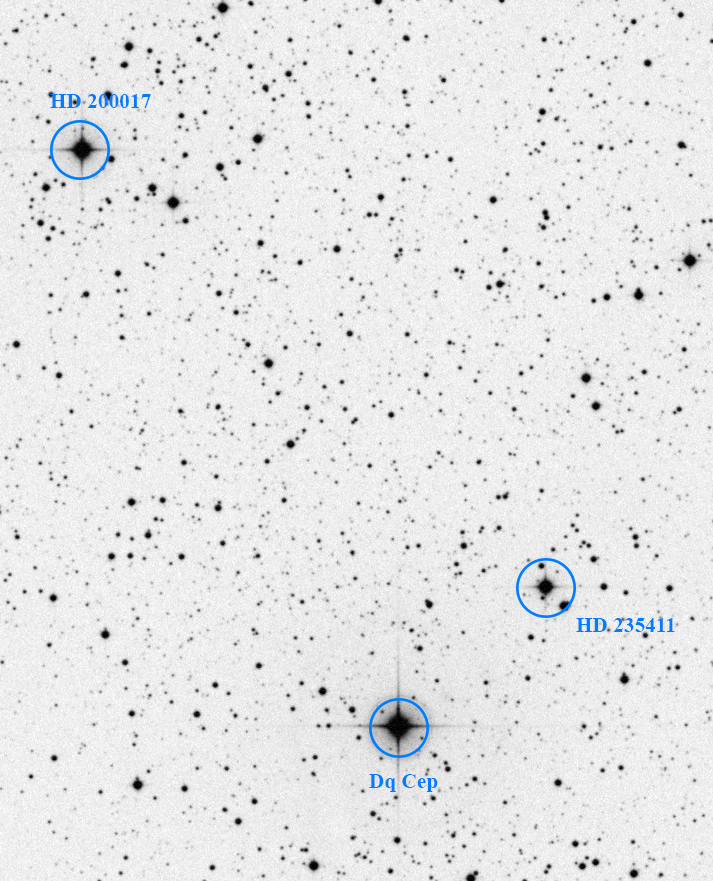
\includegraphics[width=\textwidth]{figs/dss_map.png}
		\caption{DSS Image\footnotemark}
	\end{subfigure}
	\qquad
	\begin{subfigure}[]{.45\textwidth}
		\centering
		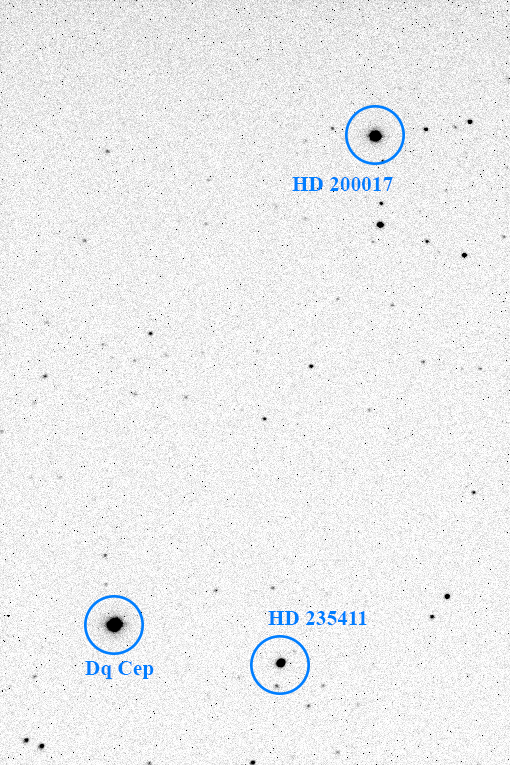
\includegraphics[width=\textwidth]{figs/map.png}
		\caption{Our image with pixel scale \numrange{200}{400}}
	\end{subfigure}
	\caption{Images showing the location of our target and reference stars using DSS and from Zaffarano Observing Deck}
	\label{fig:map}
\end{figure}
\footnotetext{The Second Palomar Observatory Sky Survey (POSS-II) was made by the California Institute of Technology with funds from the National Science Foundation, the National Geographic Society, the Sloan Foundation, the Samuel Oschin Foundation, and the Eastman Kodak Corporation.}
\begin{figure}[H]
	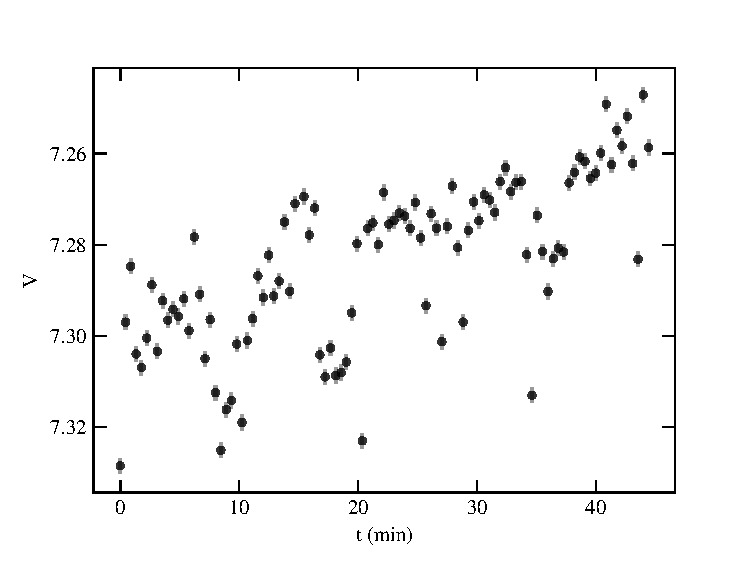
\includegraphics[width=\linewidth]{figs/mags.pdf}
	\caption{The magnitude for DQ Cep over a 45 minute period (100 images) shows a clear change in magnitude}
	\label{fig:mags}
\end{figure}
\begin{figure}[H]
	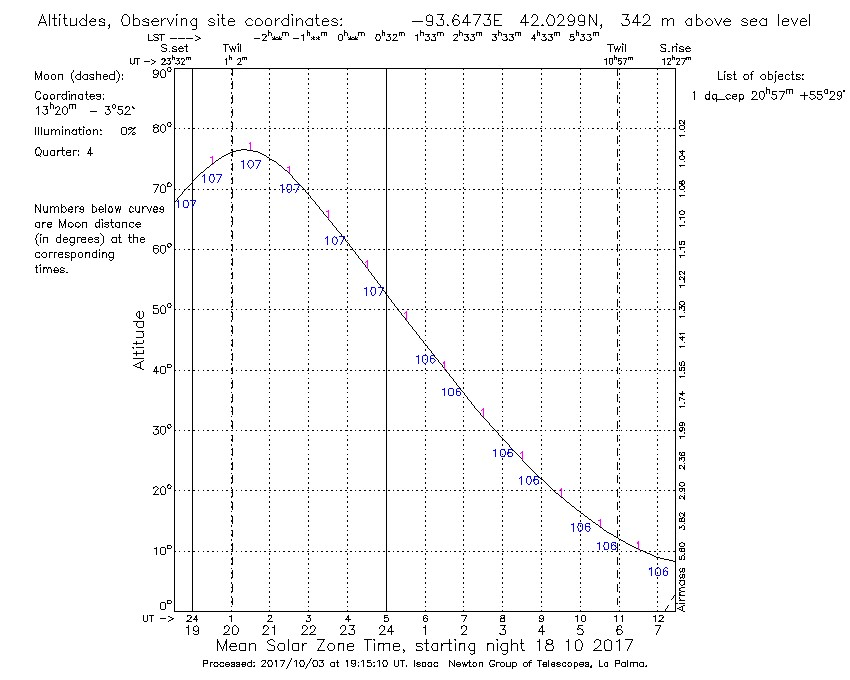
\includegraphics[width=\linewidth]{figs/staralt.png}
	\caption{Output from \textcite{staralt} Object Visibility applet . Peak is around 20:00:00 CST and is still sufficiently high four hours later at 24:00:00 CST}
	\label{fig:staralt}
\end{figure}




\end{document}
